\documentclass[12pt]{article}

\usepackage{sbc-template}
\usepackage{graphicx,url}
\usepackage[utf8]{inputenc}
\usepackage[brazil]{babel}
\usepackage[latin1]{inputenc}  
\def\code #1{\texttt{#1}}
\def\codeIndent{60pt}
     
\sloppy

\title{Relatório do Trabalho 1 de Redes\\ 2018.2}

\author{Vinicius Mascarenhas\inst{1}}

\address{Núcleo de Comptação Eletrônica (NCE) -- Universidade Federal do Rio de Janeiro (UFRJ)\\
Av. Athos da Silveira Ramos -- Cidade Universitária -- 21941-590 -- Rio de Janeiro -- RJ -- Brasil
\email{v.01110110@gmail.com}
}

\begin{document} 

\maketitle

\begin{resumo} 
Este relatório se refere a um trabalho da disciplina de Redes, ministrada pelo prof. Claudio Miceli de Farias. O trabalho em questão consiste na concepção e implementação de um protocolo de comunicação entre cliente e servidor para geração de um hipotético documento de estudante.
\end{resumo}

\section{O Princípio}

Inicialmente, a turma havia definido o protocolo como uma troca de mensagens de texto (strings) com múliplas linhas, encabeçadas por palavras-chave em caixa alta e um padding que, somado àquelas, completaria 16 caracteres no início de cada linha (0 a 15), efetivamente marcando o início do payload de cada comando na posição 16. Exemplo de mensagem de solicitação que o cliente enviaria, com o CPF como dado utilizado para seleção de registro:

\noindent\code{
\hspace*{\codeIndent}GET\ \ \ \ \ \ \ \ \ \ \ \ XXX.XXX.XXX-XX\\
\hspace*{\codeIndent} TAMANHO\ \ \ \ \ \ \ \ XX\\
\hspace*{\codeIndent} PASSWORD\ \ \ \ \ \ \ ***********\\
}

A resposta do servidor variaria de acordo com múltiplos critérios, como o preenchimento de um CPF (i.e. não deixado em branco), a existência deste valor no banco de dados, a corretude da respectiva senha, o status ativo na matrícula, a existência de um arquivo de foto do indivíduo, etc. De maneira geral, a primeira linha da resposta simularia o protocolo HTTP para que seja o mesmo protocolo utilizado em um eventual acesso via página web; e os demais dados, se autorizados, seriam passados a seguir, mantendo o mesmo padrão de estilo que a mensagem de solicitação.

\noindent\code{
\hspace*{\codeIndent}STATUS\ \ \ \ \ \ \ \ \ \ 0\ OK\\
\hspace*{\codeIndent} CURSO\ \ \ \ \ \ \ \ \ \ \ XXX\\
\hspace*{\codeIndent} DRE\ \ \ \ \ \ \ \ \ \ \ \ \ XXXXXXXXX\\
\hspace*{\codeIndent} NASC\ \ \ \ \ \ \ \ \ \ \ \ DDMMYYYY\\
\hspace*{\codeIndent} TAMANHO	\ \ \ \ \ \ \ \ XX\\
\hspace*{\codeIndent} NOME\ \ \ \ \ \ \ \ \ \ \ \ Fulano de Tal e Qual\\
\hspace*{\codeIndent} FOTO\ \ \ \ \ \ \ \ \ \ \ \ [foto em bytes]\\
}	

O campo de curso seria um número; o cliente deveria ter a informação salva para imprimir o nome do curso no documento. O campo de tamanho se refere ao número de bytes ocupados pelo nome e pela foto, para garantir a transmissão segura desses dados.
	
No entanto, devido à facilidade de comunicação via objetos passados por formulários em uma página web que o Flask fornece, a turma descartou o protocolo previamente definido, passando, portanto, a utilizar o padrão HTML. Sendo assim, todos os frontends foram desenvolvidos com páginas web em mente.

\section{O Sistema}

O código foi escrito em Python 3, com o benefício do framework Flask, em um terminal rodando \code{vim}. Foram criados um arquivo servidor.py e um registros.py, na raíz do projeto; e os seguintes templates no diretório templates: index.html, documento.html, e erro.html. As fotos de usuários ficam no diretório fotos.

O script servidor.py renderiza uma página de login com o template index.html, recebe os parâmetros passados pelo formulário, e realiza uma série de validações (Figura 1). CPF deve estar preenchido, senha deve estar correta, o usuário solicitado deve ter foto salva na pasta com o nome correto (F concatenado com o CPF e a extensão .png), e deve ter matrícula ativa. Passando em todas as validações, o programa gera um QR Code (cujo conteúdo é o CPF, para poupar futuras e repetidas digitações) e renderiza a carteirinha utilizando o template documento.html, embutindo na página tanto a foto salva como o QR Code, cujo conteúdo é o CPF para poupar digitações repetidas no futuro (Figura 2).

Em caso de erro em qualquer teste, a página renderizada com o template erro.html é criada com uma string que diz qual foi o erro, para que se possa tomar a devida providência. Os erros implementados são: CPF inválido quando é deixado em branco ou não consta dos registros (Figura 3), senha incorreta quando deixada em branco ou diferente da que está associada ao CPF (Figura 4), usuário sem foto (Figura 5), e matrícula inativa (Figura 6).

Tanto o CPF como a senha foram deixados em texto plano porque implementação de criptografia não era o objetivo do trabalho. Entretanto, são passados através do método POST para que não sejam visíveis na URL da página atingida (documento.html ou erro.html). Os dados retornados pelo servidor são incorporados à página através do uso de \code{ \{\{ templates \} \} } presentes nos respectivos arquivos HTML. Cabe notar que a informação de curso como string agora fica no lado do servidor -- não é mais passado um número para que o cliente se responsabilize por procurar a string.

\begin{figure}[ht]
\centering
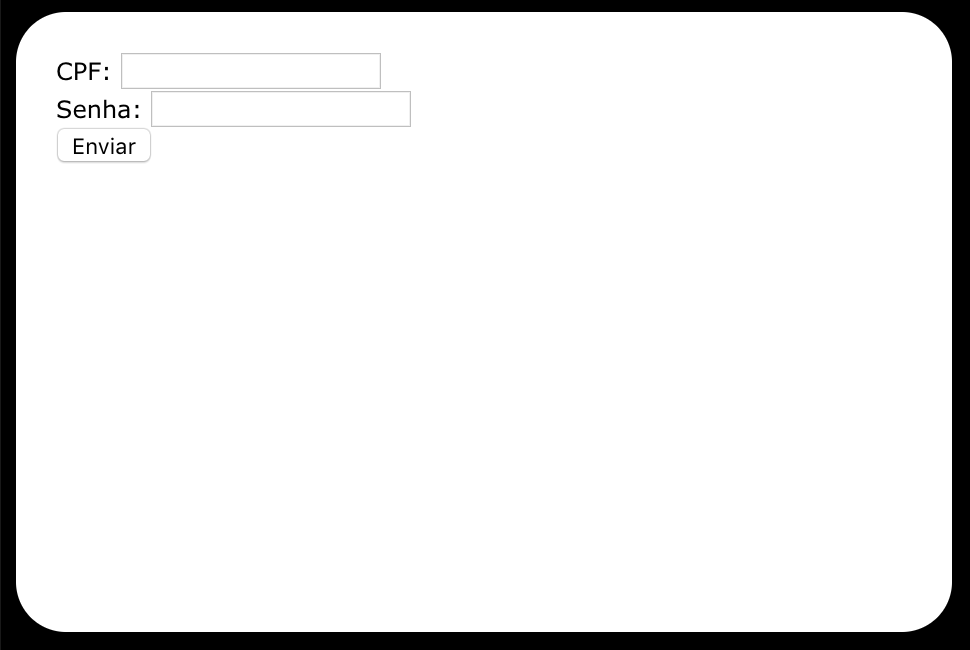
\includegraphics[width=.5\textwidth]{fig1.png}
\caption{Página de login (index.html)}
\label{fig:exampleFig1}
\end{figure}

\begin{figure}[ht]
\centering
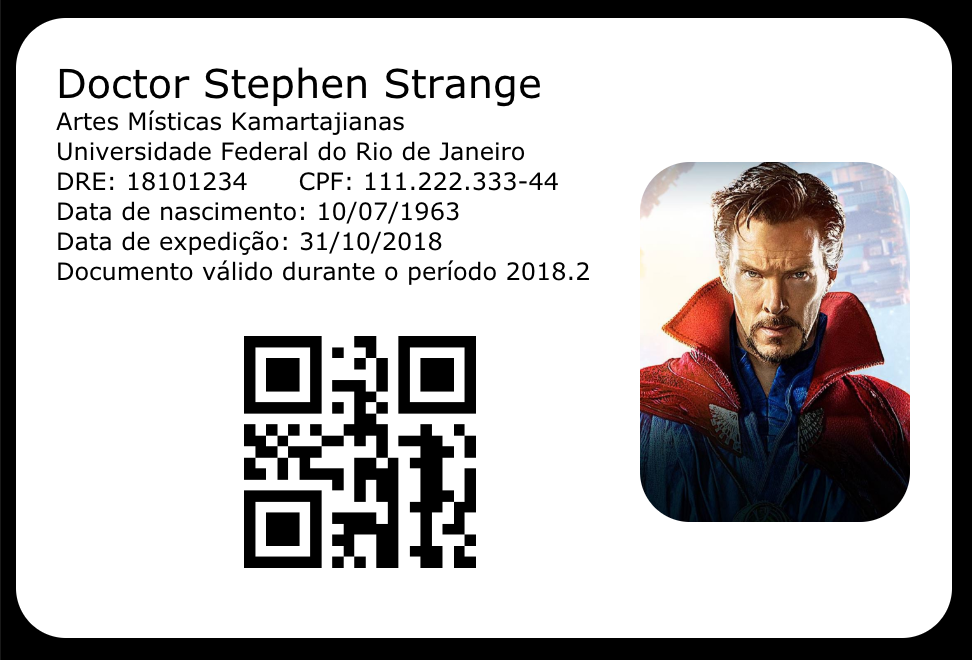
\includegraphics[width=.5\textwidth]{fig2.png}
\caption{Documento de estudante gerado (documento.html)}
\label{fig:exampleFig2}
\end{figure}

\begin{figure}[ht]
\centering
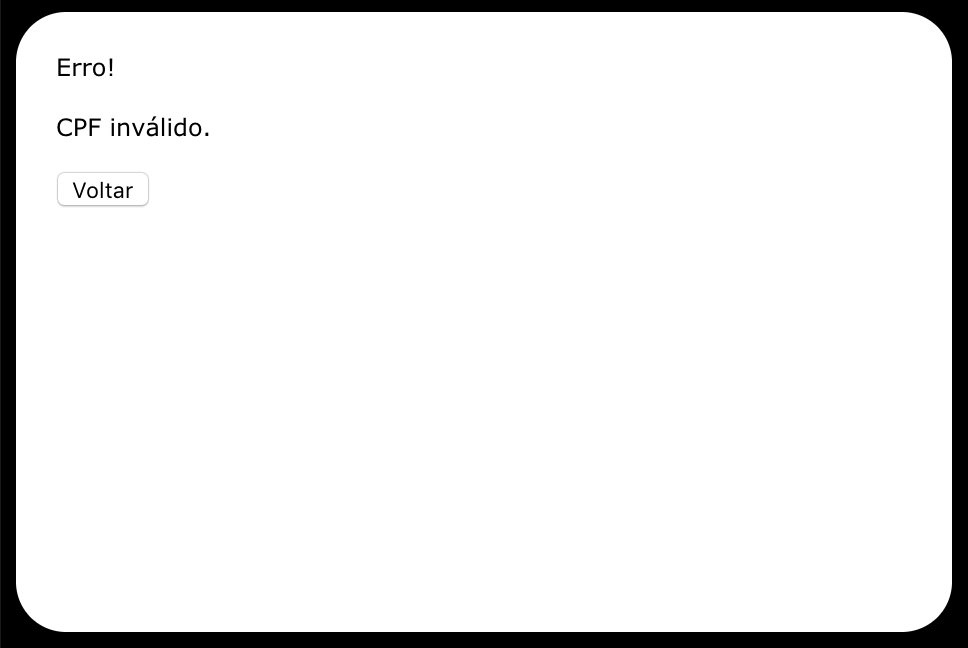
\includegraphics[width=.5\textwidth]{fig3.png}
\caption{Exemplo de erro de CPF (erro.html)}
\label{fig:exampleFig3}
\end{figure}

\begin{figure}[ht]
\centering
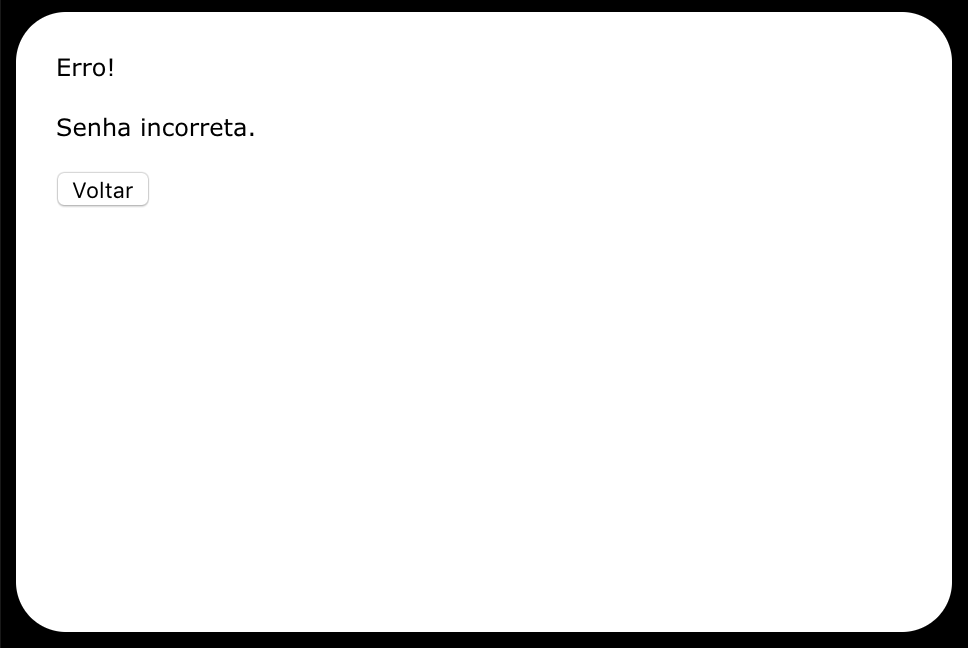
\includegraphics[width=.5\textwidth]{fig4.png}
\caption{Exemplo de erro de senha (erro.html)}
\label{fig:exampleFig4}
\end{figure}

\begin{figure}[ht]
\centering
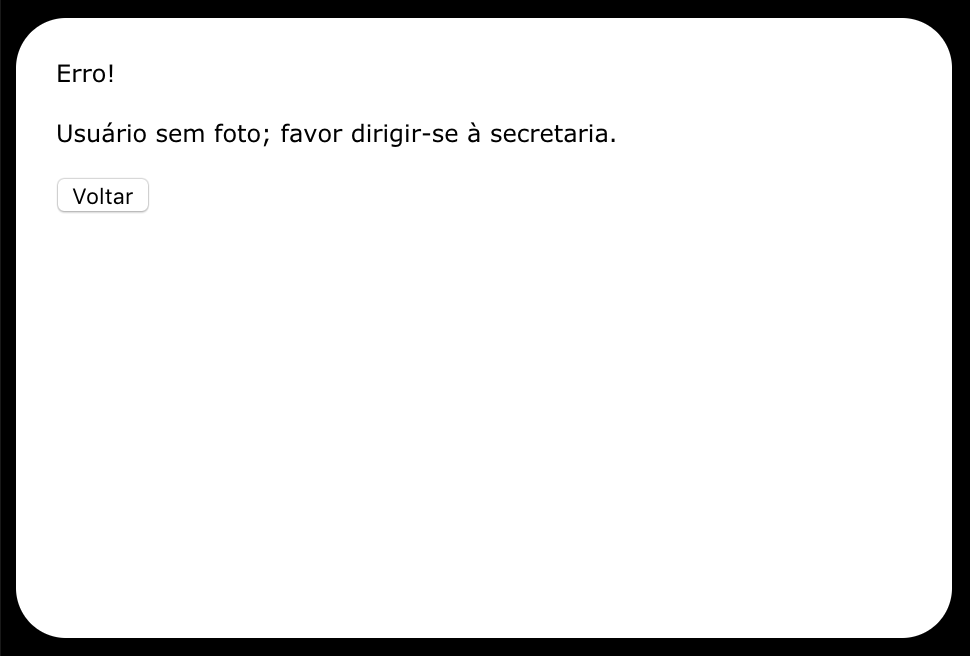
\includegraphics[width=.5\textwidth]{fig5.png}
\caption{Exemplo de erro de foto (erro.html)}
\label{fig:exampleFig5}
\end{figure}

\begin{figure}[ht]
\centering
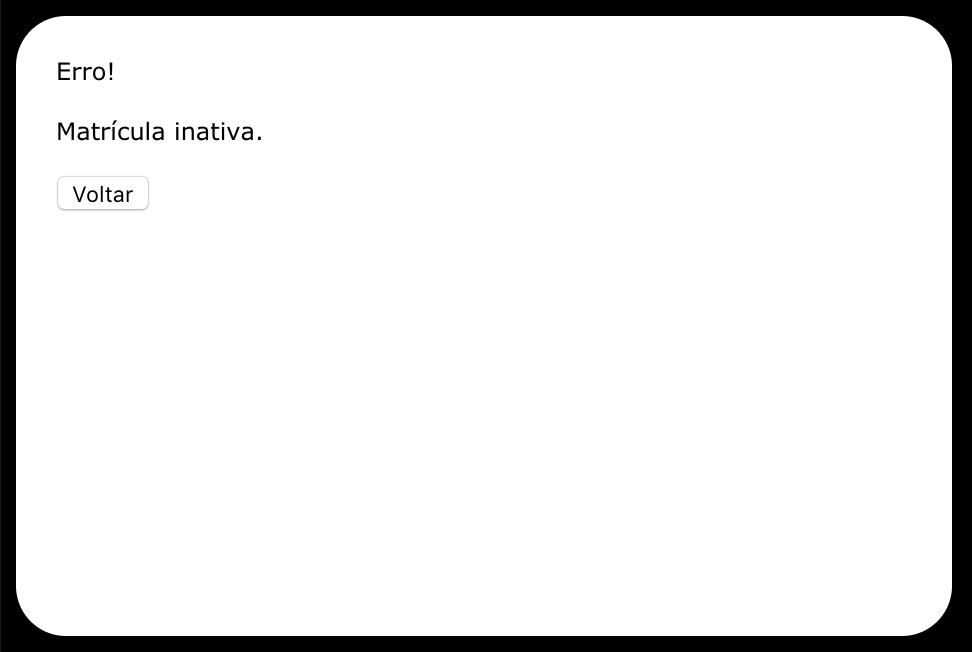
\includegraphics[width=.5\textwidth]{fig6.png}
\caption{Exemplo de erro de matrícula inativa (erro.html)}
\label{fig:exampleFig6}
\end{figure}

\end{document}
